\begin{figure}
  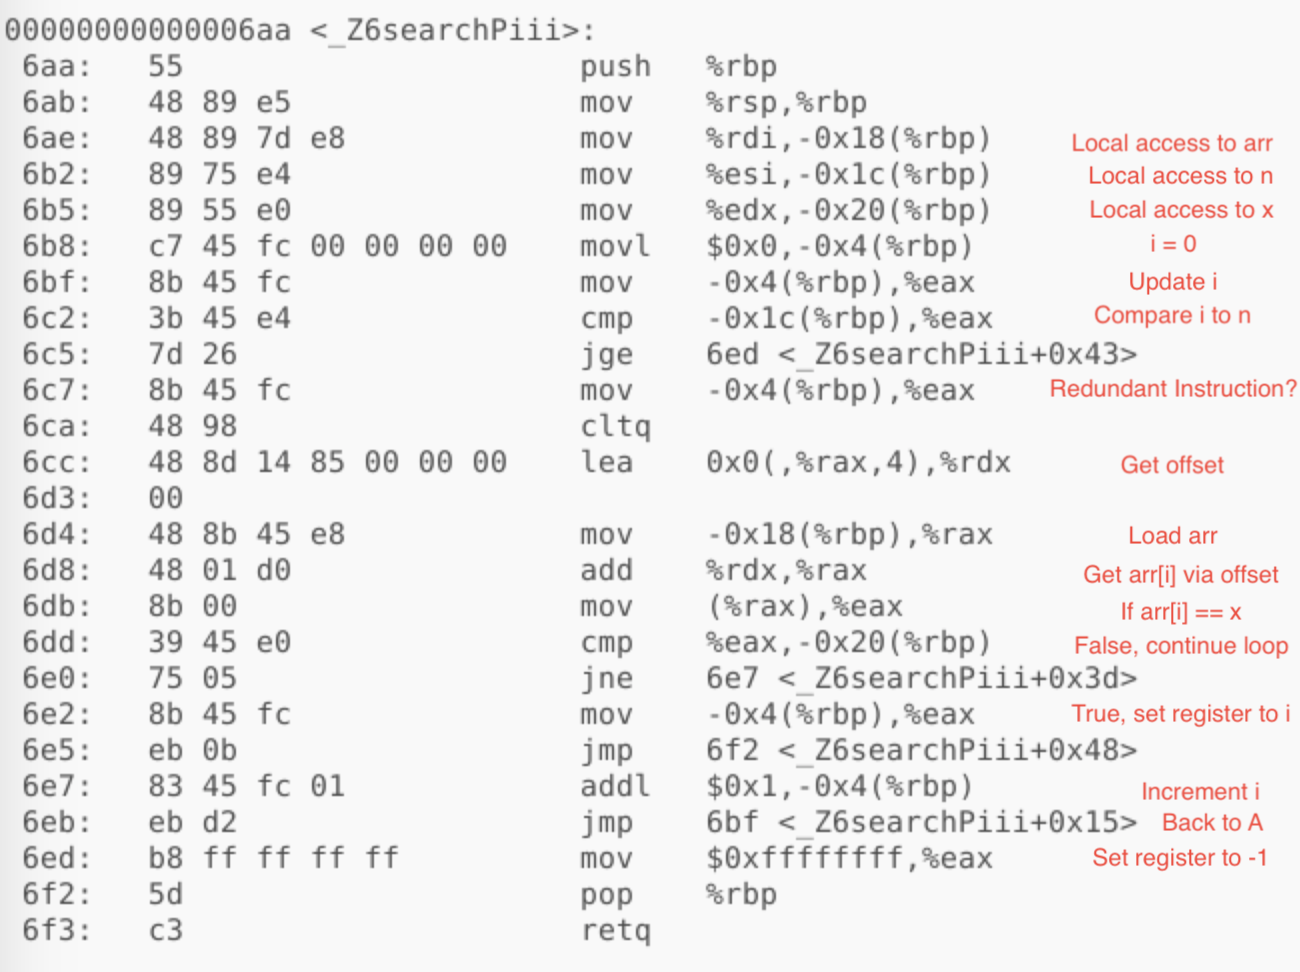
\includegraphics[width=\linewidth]{./figures/Annotated_search_assembly_ATT.png}
  \caption{Annotated version of Linear Search's search function in assembly. Similarities were found in sorting functions with the primary difference being sections of data modification and multiple for-loops.}
  \label{fig:search}
\end{figure}

Before moving towards a specific model, we first wished to see what differences occur between programs with different purposes, such as sorting programs versus searching programs. These two types of programs are two fundamental concepts of many programs and were identified as appropriate vehicles to develop and understand this approach. Initial analyses were performed on a small dataset collected from the Geeks4Geeks Website \cite{geeks}, where C++ samples of major sorting and searching algorithms were downloaded and compiled onto a Ubuntu 64-bit system. A larger dataset was later utilized using ByteWeight's dataset \cite{bao2014byteweight}. 

To understand the differences between programs, we first closely examined one sorting and one searching program to see what differences might exist between their assemblies. Figure \ref{fig:search} shows an annotated version of Linear Search's search function, and when compared with a sorting program such as Selection Sort (which effectively contains a modified version of a linear search as it sorts the program), the primary differences found were multiple for-loops and sections for data modification, something which most, if not all, sorting programs should have, but no realistic searching programs should have, as efficient searching programs should only have one loop, and should not be modifying the data. This formed the basis of our argument: \textit{Programs can be thought of as being made up of a set of underlying components, and these components are in some way shared across all programs.} The order and frequency in which these components occur can enable behavioral comparisons between programs, and understanding the components themselves allows for fine-grain understanding of behavior. The system presented in this work only incorporates the commands themselves so that basic functionality of the software could be understood. Incorporating arguments would allow for a better understanding of command targets (such as specific registers or functions), but would first require abstracting these in a way similar to Symbolic Execution so that program-to-program comparisons can be maintained.
